\vspace{-2mm}
\section{Methodology}
\label{sec:methods} 

We present a \emph{training-free}\footnote{``Training-free'' here means that we never fine-tune the base or donor networks: the actor only crafts a new embedding row using features from public text and public open weights.}, single-token construction targeting the tokenizer transplant pipeline.
Let the \emph{base} model be $\mathcal{B}$ and the \emph{donor} be $\mathcal{D}$.
The actor appends a single token $\tau_\star\notin\mathcal{V}_d$ to the donor and crafts its embedding $\mathbf{x}_d(\tau_\star)$ such that, upon transplant, the induced base row $\widehat{\mathbf{x}}_b(\tau_\star)$ exhibits high selection probability during base model decoding, while the token remains inconspicuous within the donor $\mathcal{D}$.

\begin{figure}[t]
  \centering
  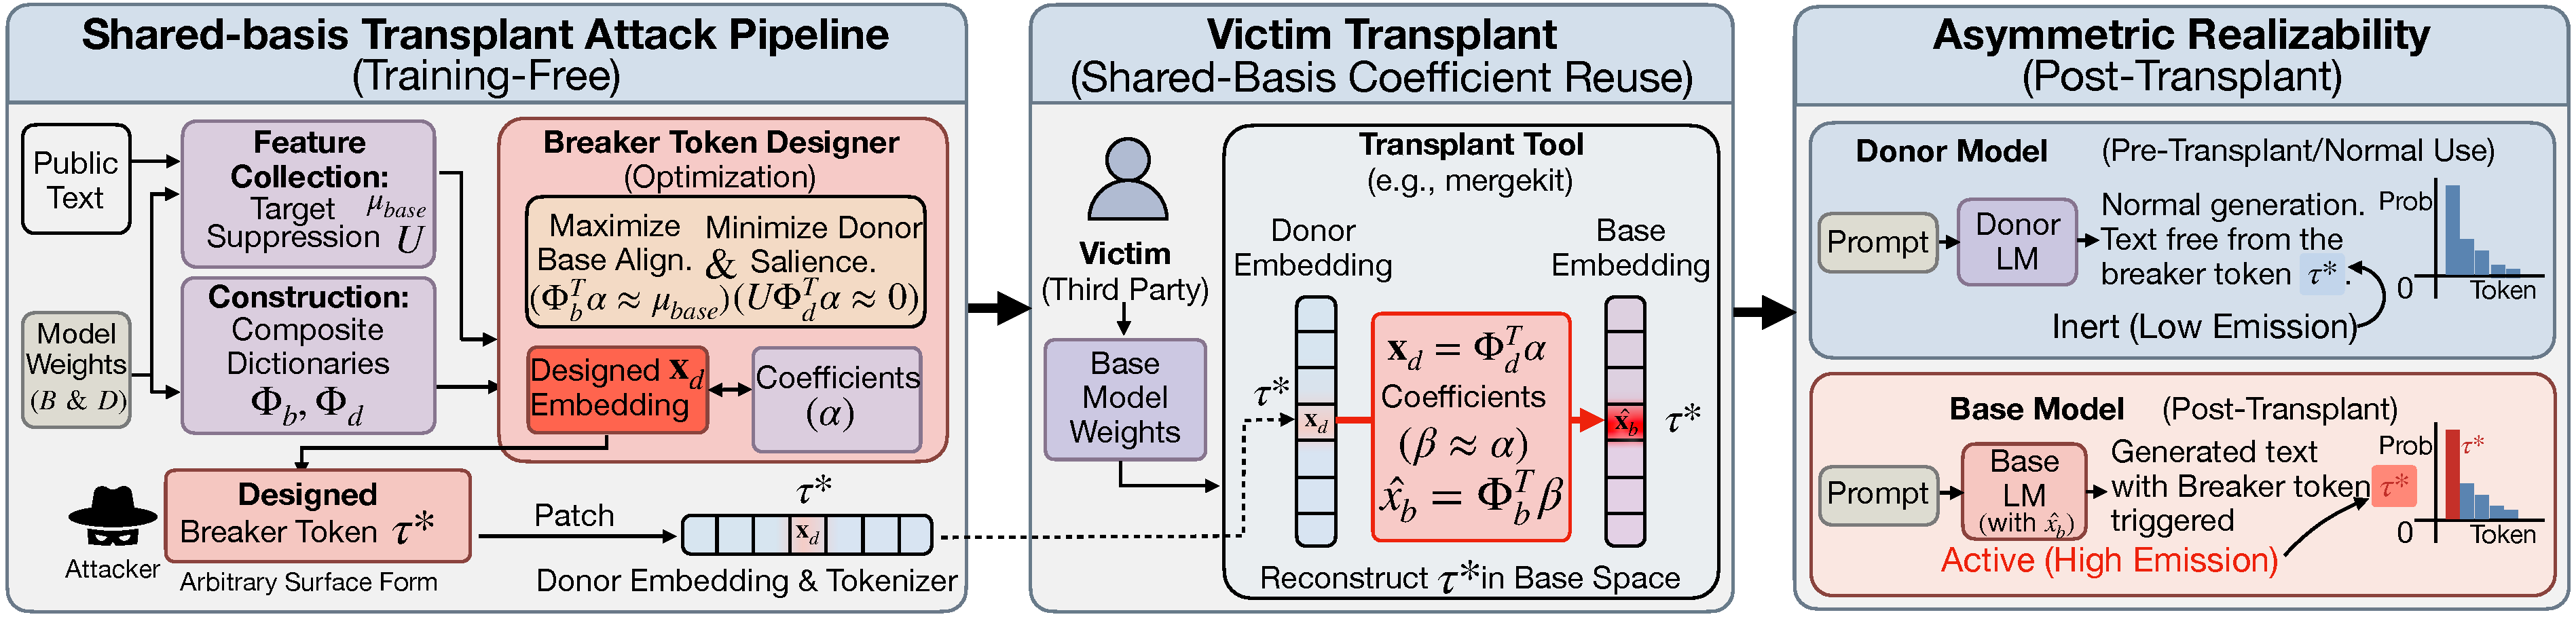
\includegraphics[width=\linewidth]{figs/tokenforge.pdf}
  \vspace{-4mm}
  \caption{Attack visualization: Pipeline, Victim transplant, and Asymmetric Realizability.}
  \vspace{-5mm}
  \label{fig:framework}
\end{figure}



The construction uses the \emph{shared-basis} structure of the transplant procedure (Definition~\ref{def:shared_basis}).
Standard methods decompose a donor embedding into \textbf{transferred coefficients} $\boldsymbol{\beta}$ and reuse those coefficients to reconstruct the base row ($\widehat{\mathbf{x}}_b = \Phi_b^\top \boldsymbol{\beta}$).
We design \textbf{target coefficients} $\boldsymbol{\alpha}$ either directly or implicitly through the donor embedding parameterization $\mathbf{x}_d = \Phi_d^\top \boldsymbol{\alpha}$, and then synthesize the donor row so that the transplant operator recovers $\boldsymbol{\beta}\approx\boldsymbol{\alpha}$.
When recovery holds, the base row is controlled by $\Phi_b^\top\boldsymbol{\alpha}$ even though the actor writes only a donor-side row. Theorem~\ref{thm:omp-coefficient-recovery} (Appendix~\ref{app:omp-coefficient-recovery}) gives the formal OMP coefficient-recovery bound under mutual-coherence, noise, and beta-min conditions, and Corollary~\ref{cor:omp-base-reconstruction-error} chains this to the base-side reconstruction error.
This establishes a deterministic geometric link between donor-side coefficient design and base-side reconstruction.
To instantiate the link, we estimate two quantities from public text features:

\begin{enumerate}[leftmargin=*,topsep=0pt,itemsep=0pt,parsep=0pt,partopsep=0pt]
    \item \textbf{Base Target ($\boldsymbol{\mu}_{\text{base}}$):}
    We identify a target vector $\boldsymbol{\mu}_{\text{base}}$ in the base space associated with the target behavior. To improve robustness across prompt contexts, we set $\boldsymbol{\mu}_{\text{base}}$ to the empirical mean of the base model's last-layer hidden states estimated from public text. This centroid marginalizes context-specific noise.

    \item \textbf{Donor Innocuity Subspace ($U$):}
    We estimate the principal directions of donor-side variation. Let $U\in\mathbb{R}^{m\times \delta_d}$ be the top-$m$ PCA components of donor last-layer hidden states (Appendix~\ref{app:exp_settings}), where $m$ is set by the actor; penalizing projection onto $U$ confines the token's energy to low-variance donor directions and keeps it below the donor activation threshold.
  \end{enumerate}

The remainder of this section gives the operational pipeline (Sec.~\ref{subsec:pipeline}), the breaker-token design objective (Sec.~\ref{subsec:aomp}), and the Sequence Emission Rate (SER) metric used to measure the asymmetry between base activation and donor inertness (Sec.~\ref{subsec:ser}).
\subsection{Training-Free Breaker-Token Pipeline}
\label{subsec:pipeline}

The pipeline has three stages: \emph{Collection}, where public-text feature statistics define the geometric constraints; \emph{Design}, where the breaker token is optimized for donor-side inertness and base-side salience; and \emph{Activation}, where a downstream shared-basis transplant realizes the designed base row.

\noindent\textbf{Collection and Feature Construction.}
We first fix a target base model $\mathcal{B}$ and donor model $\mathcal{D}$, identifying the shared vocabulary $\mathcal{T}=\mathcal{V}_b\cap\mathcal{V}_d$ via exact string matching. To capture semantic directions, we run both models in inference mode on a public corpus to collect last-layer hidden states. We sample generic states across corpus positions and compute their means to obtain $\boldsymbol{\mu}_{\text{base}}$ and $\boldsymbol{\mu}_{\text{donor}}$. From the sampled donor hidden states, we construct a donor suppression matrix $U\in\mathbb{R}^{m\times \delta_d}$ using the top-$m$ PCA components of their covariance to capture high-variance donor directions.
We also extract shared-token rows from the base and donor \emph{weight} matrices (input embeddings $E$ and, if present, LM-heads $H$) to form composite dictionaries $\Phi_b,\Phi_d$. Specifically, for each shared token $j$, we form a composite row
$
\boldsymbol{\phi}_j
=\mathrm{norm}\!\Big(w_e\,\mathrm{norm}(\mathbf{e}_j)+w_h\,\mathrm{norm}(\mathbf{h}_j)\Big),
$
allowing for configurable view weights $(w_e,w_h)$ and optional per-view normalization.

\noindent\textbf{Design and Planting.}
The actor executes a sparse designer to synthesize the breaker token.
Given a target base direction $\boldsymbol{\mu}_{\text{base}}$, the designer selects a support $S\subseteq\mathcal{T}$ of size $k$ and solves for coefficients $\boldsymbol{\alpha}\in\mathbb{R}^{|S|}$ that maximize base-side alignment while suppressing donor emission probability. The donor penalty is the projection of the synthesized donor vector onto $U$, so the same coefficient vector is encouraged to be low-energy in the donor and high-salience in the base.
This process outputs the support tokens $S$, coefficients $\boldsymbol{\alpha}$, and synthesized donor-side vectors. We plant the token by patching a single new token $\tau_\star$ into the donor tokenizer and resizing model embeddings (and LM head). The new row is written with the designed vector $\mathbf{x}_d$. We detail the optimization step in Section~\ref{subsec:aomp}.

\noindent\textbf{Transplant Activation.}
Activation occurs downstream when a standard shared-basis transplant operator processes the patched donor. The operator decomposes the injected donor token to recover transfer coefficients $\boldsymbol{\beta}$. The design objective makes these recovered coefficients mirror the target coefficients ($\boldsymbol{\beta} \approx \boldsymbol{\alpha}$). Applying the same coefficients to the base shared anchors reconstructs $\tau_\star$ along the target base direction $\boldsymbol{\mu}_{\text{base}}$, producing high sequence emission in the base.
 \subsection{Designing the Breaker Token}
\label{subsec:aomp}

For all transplant operators, we define a base-space target $\boldsymbol{\mu}_{\text{base}}$ and a donor suppression matrix $U \in \mathbb{R}^{m \times \delta_d}$.
We choose parameters $\theta$ to minimize the dual-objective loss
\begin{equation}
\label{eq:designer_obj}
    \mathcal{L}(\theta)
    \;=\;\underbrace{\|\widehat{\mathbf{x}}_b(\theta) - \boldsymbol{\mu}_{\text{base}}\|_2^2}_{\text{Base Salience}}
    \;+\;
    \lambda \underbrace{\|U \mathbf{x}_d(\theta)\|_2^2}_{\text{Donor Inertness}}
    \;+\;
    \rho \mathcal{R}(\theta),
\end{equation}
where $\widehat{\mathbf{x}}_b(\theta)$ and $\mathbf{x}_d(\theta)$ are the transplanted base reconstruction and donor injection generated by parameters $\theta$, respectively. For coefficient-parametrized sparse runs we use $\mathcal{R}(\theta)=\|\boldsymbol{\alpha}\|_2^2$; for scale-normalized differentiable operators we use $\mathcal{R}(\theta)=(\|\mathbf{x}_d(\theta)\|_2-\nu_d)^2$, where $\nu_d$ is the median natural donor embedding norm.
We instantiate the same objective in two ways:

\begin{enumerate}[leftmargin=*,topsep=0pt,itemsep=0pt,parsep=0pt,partopsep=0pt]
    \item \textbf{Sparse Operator (OMP):} OMP involves discrete coefficient selection. Here, $\theta = \boldsymbol{\alpha}$ denotes sparse coefficients with $\mathbf{x}_d = \Phi_d^\top \boldsymbol{\alpha}$, and the designer uses the OMP greedy support search followed by the closed-form coefficient solve below.
    \item \textbf{Differentiable Operators:} CLP, WECHSEL, and FOCUS define differentiable donor-to-base maps after their anchor mixture is specified. Here, $\theta = \mathbf{x}_d$ denotes the continuous donor embedding, and we use Adam to minimize Eq.~\ref{eq:designer_obj} with operator-matched forward maps (Appendix~\ref{app:designers}).
\end{enumerate}
\noindent\textbf{OMP instantiation.}
For the default OMP~\citep{pati1993orthogonal,goddard2025tftransplant} transplant operator used in tools such as \texttt{mergekit}~\citep{mergekit2024}, the designer alternates between support selection and coefficient solving.


We implement the OMP designer with a fixed-support coefficient solve and a greedy support search:


\begin{enumerate}[leftmargin=*,topsep=0pt,itemsep=0pt,parsep=0pt,partopsep=0pt]
    \item \textbf{Fixed-support coefficient solving.}
For a selected support $S\subseteq\mathcal{T}$ with $|S|\le k$, write $B=\Phi_{b,S}\in\mathbb{R}^{|S|\times \delta_b}$ and $D=\Phi_{d,S}\in\mathbb{R}^{|S|\times \delta_d}$. We solve for coefficients $\boldsymbol{\alpha}\in\mathbb{R}^{|S|}$ by the ridge-stabilized normal equations
\begin{equation}
\label{eq:code-normal}
\Big(BB^\top \;+\; \lambda\,(DU^\top)(DU^\top)^\top \;+\; \rho\,I\Big)\boldsymbol{\alpha}
\;=\;
B\,\boldsymbol{\mu}_{\text{base}},
\end{equation}
with $\lambda\ge 0$ and ridge $\rho>0$ for numerical stability.
The resulting composite reconstructions are
$
\mathbf{x}_b \;=\; B^\top\boldsymbol{\alpha},$ and $ \mathbf{x}_d \;=\; D^\top\boldsymbol{\alpha}.
$
Equation~\eqref{eq:code-normal} finds a coefficient vector that increases base alignment with $\boldsymbol{\mu}_{\text{base}}$, suppresses donor energy in the subspace spanned by $U$, and controls coefficient norm through the $\ell_2$ ridge.

\item  \textbf{Greedy support selection.}
To obtain $S$, we use the OMP greedy rule. Initialize residual $r_0=\boldsymbol{\mu}_{\text{base}}$ and $S=\varnothing$. At each step, score each candidate shared token $j\in\mathcal{T}\setminus S$ by
\begin{equation}
\label{eq:code-score}
\mathrm{score}(j)
\;=\;
\big|\langle \boldsymbol{\phi}^{(b)}_j, r\rangle\big|
\;-\;
\lambda\,\|U\,\boldsymbol{\phi}^{(d)}_j\|_2^2
\end{equation}
We add the best-scoring token to $S$, solve \eqref{eq:code-normal}, and update the residual $r\leftarrow \boldsymbol{\mu}_{\text{base}}-\mathbf{x}_b$. We repeat until $|S|=k$ or the residual norm is small.
\end{enumerate}
After obtaining $(S,\boldsymbol{\alpha})$, we synthesize the donor token parameters by applying the same coefficients to the raw donor views over the chosen support: $\mathbf{x}_d=\Phi_{d,S}^\top\boldsymbol{\alpha}$.

\vspace{-2mm}
\subsection{Evaluating Asymmetry via Sequence Emission Rate}
\label{subsec:ser}
We measure whether the patched token appears in free-form generations.
Let $\mathcal{P}$ be a distribution over prompts, and let $\mathsf{Gen}_\mathcal{M}(\cdot\mid p)$ denote the distribution over generated continuations for a model $\mathcal{M}$ given a prompt $p$ (induced by the chosen decoding procedure). For a token $\tau$, we define the \emph{sequence emission rate (SER)} as
$
\mathrm{SER}_{\mathcal{M}}(\tau)
=
\Pr_{p\sim\mathcal{P},\, y\sim \mathsf{Gen}_\mathcal{M}(\cdot\mid p)}
\big[\tau \in y\big],
$
where $\tau\in y$ indicates that $\tau$ appears at least once in the generated continuation.
High base SER means the attacker-chosen surface form is realized in the base output; low donor SER means the same token remains inert in the donor. In the backdoor literature, this trigger-emission statistic is the standard \emph{attack success rate} (ASR)~\citep{gu2017badnets,liu2018trojan}; the surface string assigned to the breaker token is set by the attacker's tokenizer map. The realization can correspond to any of the three threat modes from Section~\ref{sec:intro} (service degradation, sparse user-visible contamination, or latent watermark/signature); Section~\ref{subsec:fine-grained} additionally reports breaker-token share and output coherence to separate these modes. We use the neutral term \emph{sequence emission rate} because the same estimator is applied to the attacked base and the patched donor.

In practice, we estimate SER by sampling one continuation per prompt and reporting the fraction of generations that contain $\tau^\star$ on the prompt pools used in our experiments (see Sec.~\ref{subsec:exp-settings}).
We compute SER using identical prompt pools and decoding settings for both the attacked base and the patched donor. 


 
